%!TEX root = ../thesis.tex

% Define block styles
\tikzstyle{block} = [rectangle, draw, fill=blue!20, 
    text width=5em, text centered, rounded corners, minimum height=4em, node distance=4cm]
\tikzstyle{line} = [draw, -latex']
I
\chapter{Mobile App}
\label{sec:mobile_app}

Smart heating systems are on the rise. More and more companies are trying to secure a spot in the market offering a variety of features in their control applications, which are mostly mobile or tablet based or even come with their own device. In this section we discuss the Android application we designed and implemented for users to control our heating system. We focused on keeping things simple because as we were researching some of the already existing systems we realised very quickly that the main issue is usability. In almost all cases the user is presented with an abundance of features and extras. Even though most of them would be very useful and effective, the average user will most likely be overwhelmed. Many user interfaces put functionality first. This often results in cluttered designs. Figure \ref{fig:smart_heating_apps} shows some of the user interfaces for controlling smart heating systems.

In Section \ref{sec:use_cases} we look at some use cases for such control systems and talk about how a general control application would handle them. Afterwards we show our own design of the application for control the smart heating system we are presenting.

Because of the lack of easy to use controlling in already existing systems we chose to focus our design decisions on these aspects. The user is confronted only with a small number of screens which are all visually designed in a way so the user will always immediately know what he is looking at. The different screens are discussed in further detail in Sections \ref{sec:first_view} through \ref{sec:last_view}.

Finally we evaluate our design decisions, reflecting on the use cases to see which ones were covered by our application and which ones were not. Naturally during development we came up with a lot of new ideas for new features and extras for our own application but we decided to stick with the initial design choices to keep it as simple as possible. We will talk more about these ideas in Section \ref{sec:futurework}, where possible future work on this project is listed.

\begin{figure}
	\begin{center}
		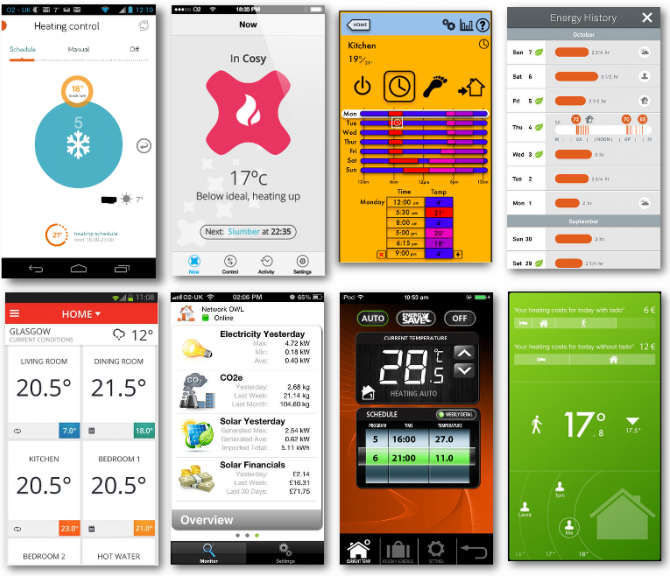
\includegraphics[width=0.8\textwidth]{images/smart_heating_apps.png}
	\end{center}
	\caption{Some examples of mobile applications for controlling smart heatings systems. Source: \url{https://cdn.recombu.com/media/digital/news/legacy/M13058/1397569835_w670_h576.png}}
	\label{fig:smart_heating_apps}
\end{figure}


\section{Use Cases}
\label{sec:use_cases}

We analyze different use cases that an average user might run into while using a smart heating system. This way we are able to ensure that our design decision leads to a simple yet effective application which helps the user control the system in an easy way without overcomplicating things. There is a tradeoff that certain functionality is lost because of these decisions but our main focus was to create an application which is easy to use. 

\begin{enumerate}
\item \textbf{Use Case: User wants to install the system}

Anna has just purchased the smart heating system in the store. After she comes home, she unwraps the components and wants to install the system. The manual tells her to install the mobile app to set up the system. The app guides her through the installation process and allows her to connect the thermostats she manually installed on the radiators to the system.
\item \textbf{Use Case: User feels cold}

Bob is sitting in the living room feeling cold. He starts the mobile app to access the temperature of for the living room. He sees that the current temperature is at 18 C and that the target temperature is 21 C. He realizes that he has already changed the temperature and notices the app tells him how much longer he has to wait for the room to heat up.
\item \textbf{Use Case: User wants to save money}

Jack is short on money. He wants to save as much as he can to get through the month, so he start the mobile app for his smart heating system. The application tells him that he can save up to 10 dollars this month by reducing the target temperature for his bathroom by five degrees. He does like it warm in the bathroom but another pair of socks will do just fine, he thinks.
\item \textbf{Use Case: User wants to add a room to an existing system}

Claire finally got her husband to agree to install the new heating system in his office as well. He does not like to deal with that tech-stuff, so Claire will take care of this. Using the already installed mobile application on her phone she can easily add another room to the system and copy the existing heating schedules.
\item \textbf{Use Case: User wants to add a thermostat to a room in the system}

When John bought his heating system he wanted to first try it out with only one of his radiators. Seeing how well the system is behaving he decides to buy new thermostats for all the radiators in his room. Gladly, adding new thermostats to an already existing system is easy using the mobile application. Soon he will save even more money on gas bills.
\item \textbf{Use Case: User feels hot}

Joe and Mary have finally gotten used to the new heating system. Mary usually feels cold very quickly, so she tends to turn the living room's target temperature up a bit too high in Joe's opinion. But this week, she is out of town and Joe can already feel the sweat running down his back, so he opens the mobile application for the heating system and sets a new target temperature for the living room. He can already hear the heater shutting down and is looking forward to a smaller bill and a more comfortable temperature.
\end{enumerate}

\section{Implementation}

\subsection{Application Flow}

As seen in Figure \ref{fig:app_flow} there are four different views in the application. These different views are explained in more detail in the following sections. The Welcome View is special, because that one is only shown when the user opens the app for the first time and has not yet registered his raspberry pi with the server. After registration, the application will always start in the Home View and go from there.

\begin{figure}[!htb]
\begin{tikzpicture}
    % Place nodes
    \node [block] (welcome) {Welcome View};
    \node [block, right of=welcome, node distance = 3cm] (home) {Home View};
    \node [block, right of=home, node distance = 5cm] (room) {Room Detail View};
    \node [block, right of=room, node distance = 5cm] (schedule) {Schedule View};
    % Draw edges
    \path [draw=black,solid,line width=1mm,preaction={-triangle 90,thin,draw,shorten >=-0.5mm}] (home) -- ([yshift=-1cm]home.south) -- ([yshift=-1cm]room.south)  node [midway, above]{Add new room} -- (room.south) ;
    \path [draw=black,solid,line width=1mm,preaction={-triangle 90,thin,draw,shorten >=-0.5mm}] (welcome) -- (home);
    \path [draw=black,solid,line width=1mm,preaction={-triangle 90,thin,draw,shorten >=-0.5mm}] (home) -- (room) node [midway, above] {Select Room};
    \path [draw=black,solid,line width=1mm,preaction={-triangle 90,thin,draw,shorten >=-0.5mm}] (room) -- (home) node [midway, below] {Back};
    \path [draw=black,solid,line width=1mm,preaction={-triangle 90,thin,draw,shorten >=-0.5mm}] (room) -- (schedule) node [midway, above] {Edit Schedule};
    \path [draw=black,solid,line width=1mm,preaction={-triangle 90,thin,draw,shorten >=-0.5mm}] (schedule) -- (room) node [midway, below] {Back};
\end{tikzpicture}
\caption{The application flow of the mobile app.}
	\label{fig:app_flow}
\end{figure}

\subsection{Welcome View}
\label{sec:first_view}
In the Welcome View, before being able to use the system the user is prompted to scan his raspberry pi in order to register it with the server. Once the registration is complete the internal database is set up according to the model seen in Figure \ref{fig:db_model}. The database is a simple model that keeps track of the rooms and thermostats which the user has added to the system so far, as well as the user's desired heating schedule for each room. To prevent any data inconsistencies, every entry in the table $Room$ has a field $server\_id$. This field corresponds to the $id$ of the room objects on the server.

\begin{figure}
	\begin{center}
		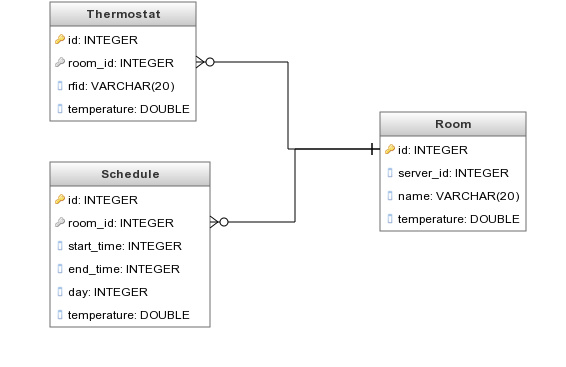
\includegraphics[width=0.8\textwidth]{images/mobile_database.jpeg}
	\end{center}
	\caption{The database model used in the mobile application.}
	\label{fig:db_model}
\end{figure}

After the initial setup of the database, the user is confronted with four questions about his daily routine. The questions are:

\begin{itemize}
\item{When do you usually wake up in the morning?}
\item{When do you usually leave for work in the morning?}
\item{When do you usually get home from work in the evening?}
\item{When do you usually go to bed in the evening?}
\end{itemize}

\begin{figure}
	\begin{center}
		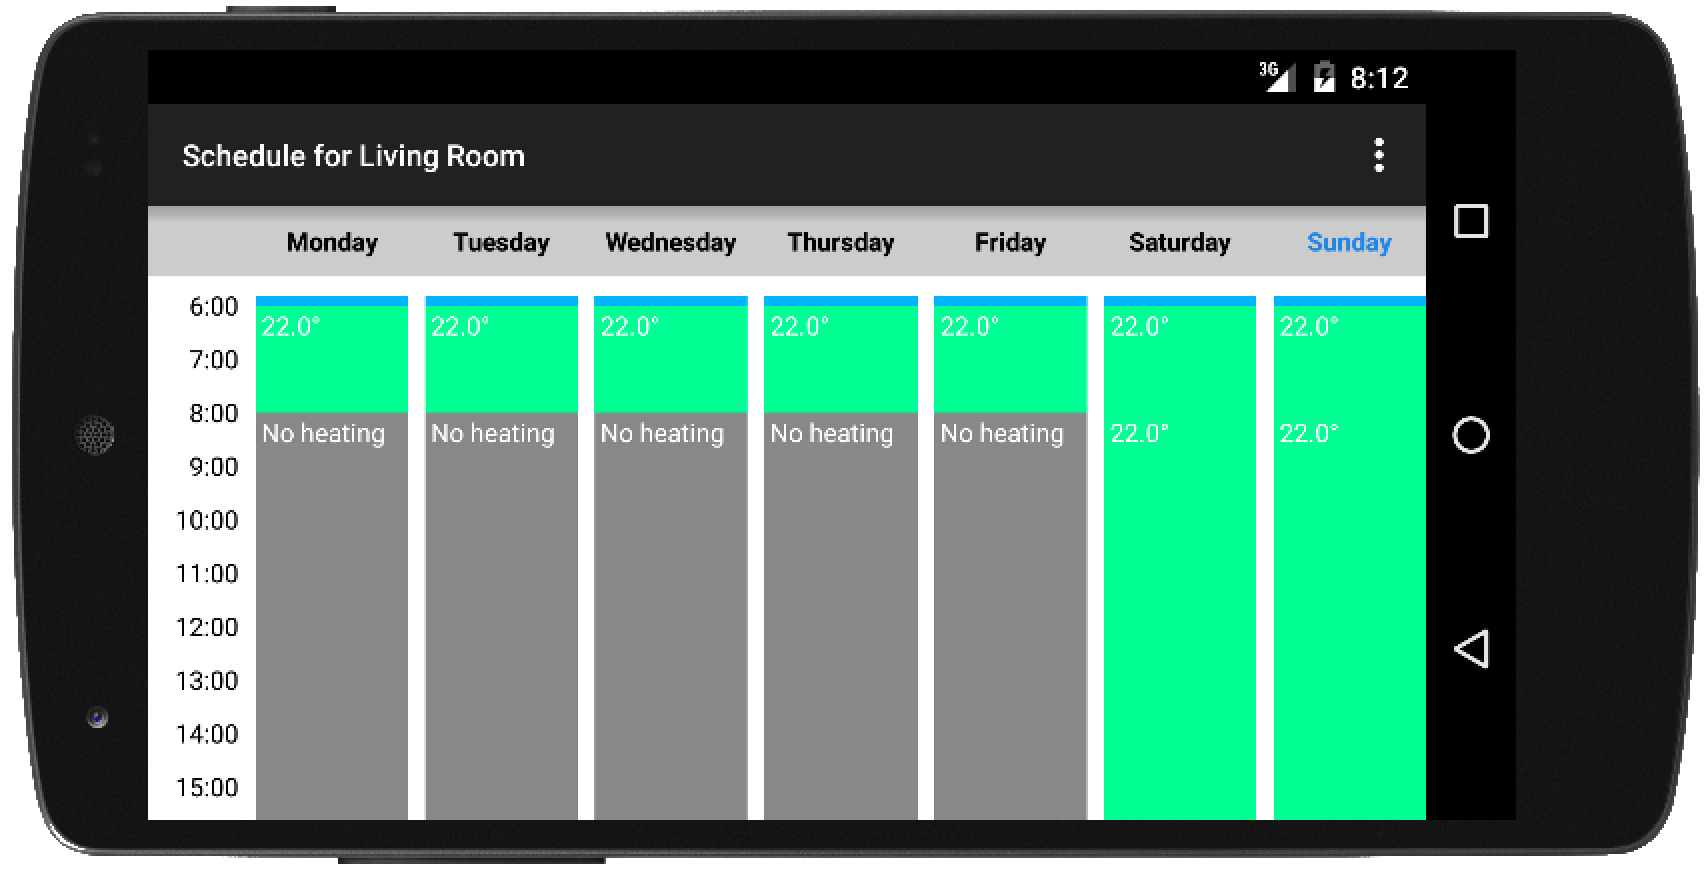
\includegraphics[width=0.8\textwidth]{images/default_heating_schedule.png}
	\end{center}
	\caption{A sample default heating schedule after the initial setup of the system.}
	\label{fig:default_schedulel}
\end{figure}

With the help of these four questions the application is able to set up a default heating schedule which is initially used for all the rooms that are added in the future. It simply takes the answers to the four questions and sets up the heating schedule in the following way: 

\begin{itemize}
\item{If the user is at home, the temperature is set to the default value for when somebody is at home.}
\item{If the user is at work, the heating is turned off completely.}
\item{If the user is sleeping, the temperature is set to the default value for the night.}
\item{On weekends, the temperature stays on the default value for being home throughout the whole day.}
\end{itemize}

These default values are initially set to 16 and 22 degrees celsius for being home and sleeping respectively.

If desired, the user can also change every heating schedule separately to his own needs. More details about heating schedules can be found in Section \ref{sec:schedule_view}.

\subsection{The Home View}
\label{sec:home_view}
The home view is where the application usually starts after successful registration of the raspberry pi with the server. In the home view the user can see all the rooms he added to the system with the corresponding current temperatures in each room. The colour of the tiles with the room names are also an indicator to how hot the room is in its current state, ranging from blue (cold) to green (normal) to red (hot). Clicking one of the tiles will lead the user to the room detail view described in Section \ref{sec:detail_view}. Next to the current temperature of each room there is an optional flame icon indicating that the room is being heated up at the moment. See Figure \ref{fig:home_view} for an example.

Via the menu in the upper righthand corner, the user can choose to add new rooms or delete existing ones. Adding a new room simply requires a new name for the room to be entered. After the creation of a new room the user is immediately transferred to the room detail view so that he can add new thermostats to the room. For more details about the room detail view see Section \ref{sec:detail_view}.

\begin{figure}
	\begin{center}
		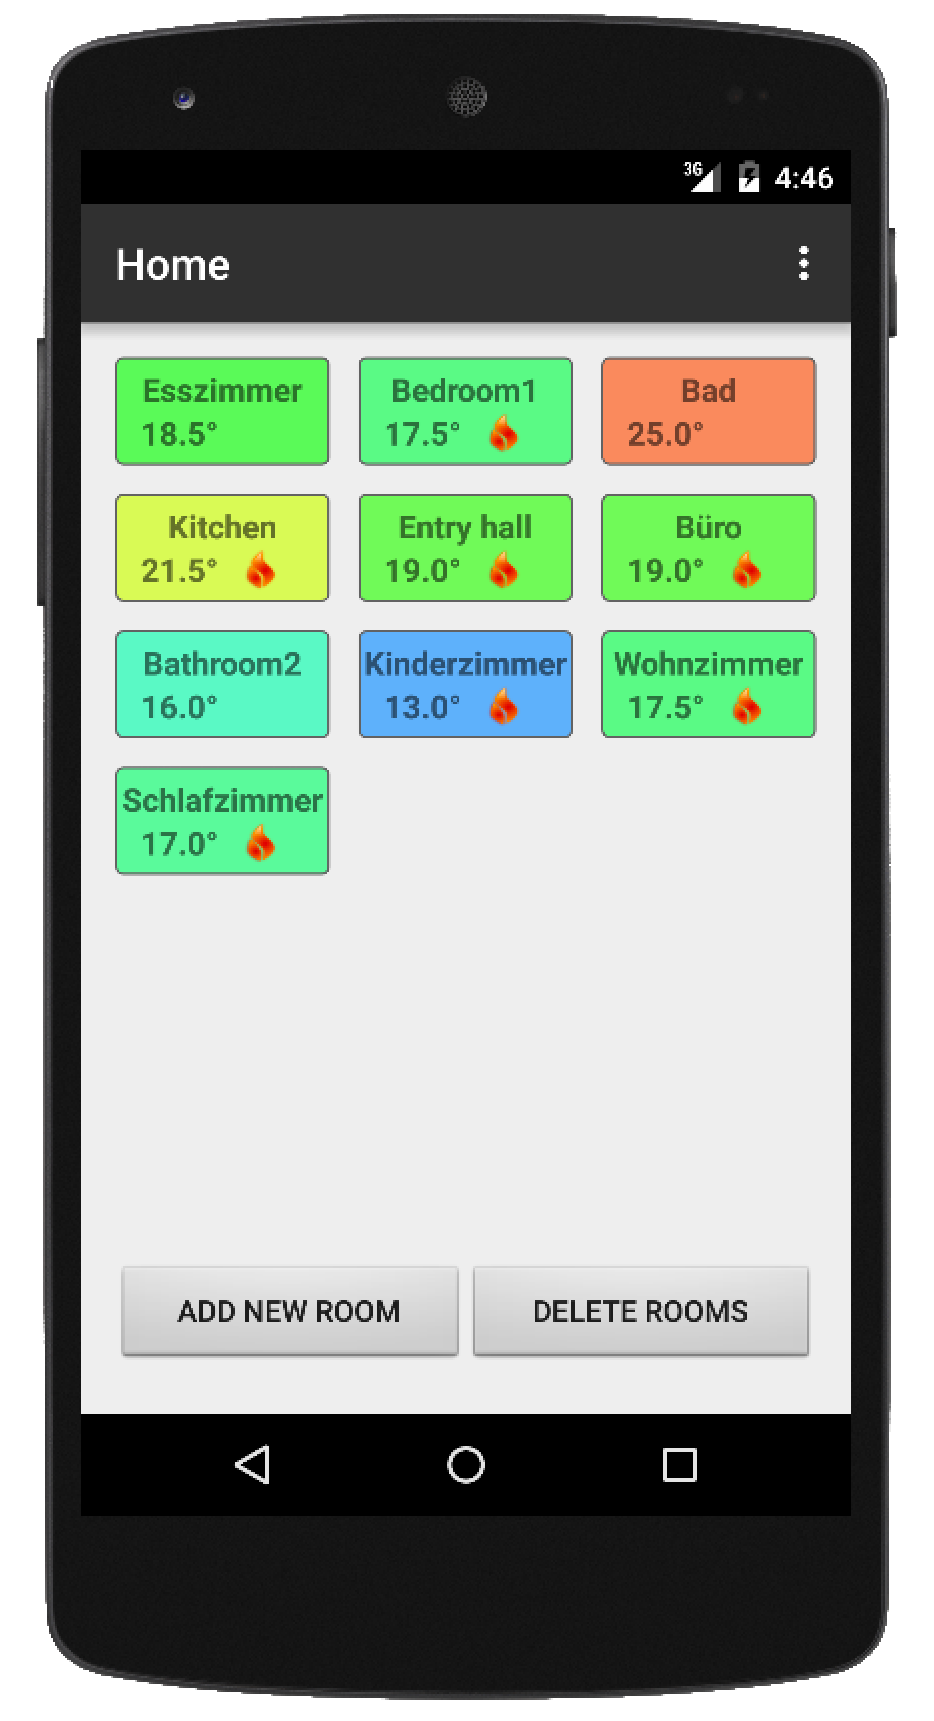
\includegraphics[width=0.8\textwidth]{images/home_view.png}
	\end{center}
	\caption{A sample home view with some random rooms.}
	\label{fig:home_view}
\end{figure}

\subsection{The Room Detail View}
\label{sec:detail_view}
After clicking one of the tiles in the home view the user is presented with more details about the room. He can see a list with all the thermostats, the current temperature in the room indicated with a large thermometer and also a slider next to it for adjusting the desired temperature of the room.

The desired temperature comes from the heating schedule currently active for the room. If the user wants to change the desired temperature he can simply drag the slider to a new position. The heating schedule for the room will be adjusted automatically as well.

If the user wants to change the heating schedule manually he can do so by selecting "View/Edit schedule" from the menu located in the upper righthand corner. This will lead him to the schedule view described further in Section \ref{sec:schedule_view}. 
\todo{picture detail view}

\subsection{The Schedule View}
\label{sec:schedule_view}
\label{sec:last_view}
The schedule view shows the heating schedule of the room the user has selected previously in the home view. The application is forced into landscape mode to be able to display all the days of the week. The current day of the week is highlighted for easier usability. The user can scroll up and down to see all the different times of the day. 

Adding a new entry is simple: with a single tap anywhere on the schedule the user can add a new entry in the corresponding time slot. He can also adjust the exact times of the new entry after tapping. After providing the desired target temperature for the new entry the user can confirm the data and the new schedule entry is sent to the local database as well as the online server right away. 

Removing a heating schedule entry is not possible and should not be necessary. If the user wants to turn off the heating for a certain period he can simply add a new entry or edit an existing one and check the "No heating" checkbox. See Figure \ref{fig:new_schedule_entry} for an example.

\begin{figure}
	\begin{center}
		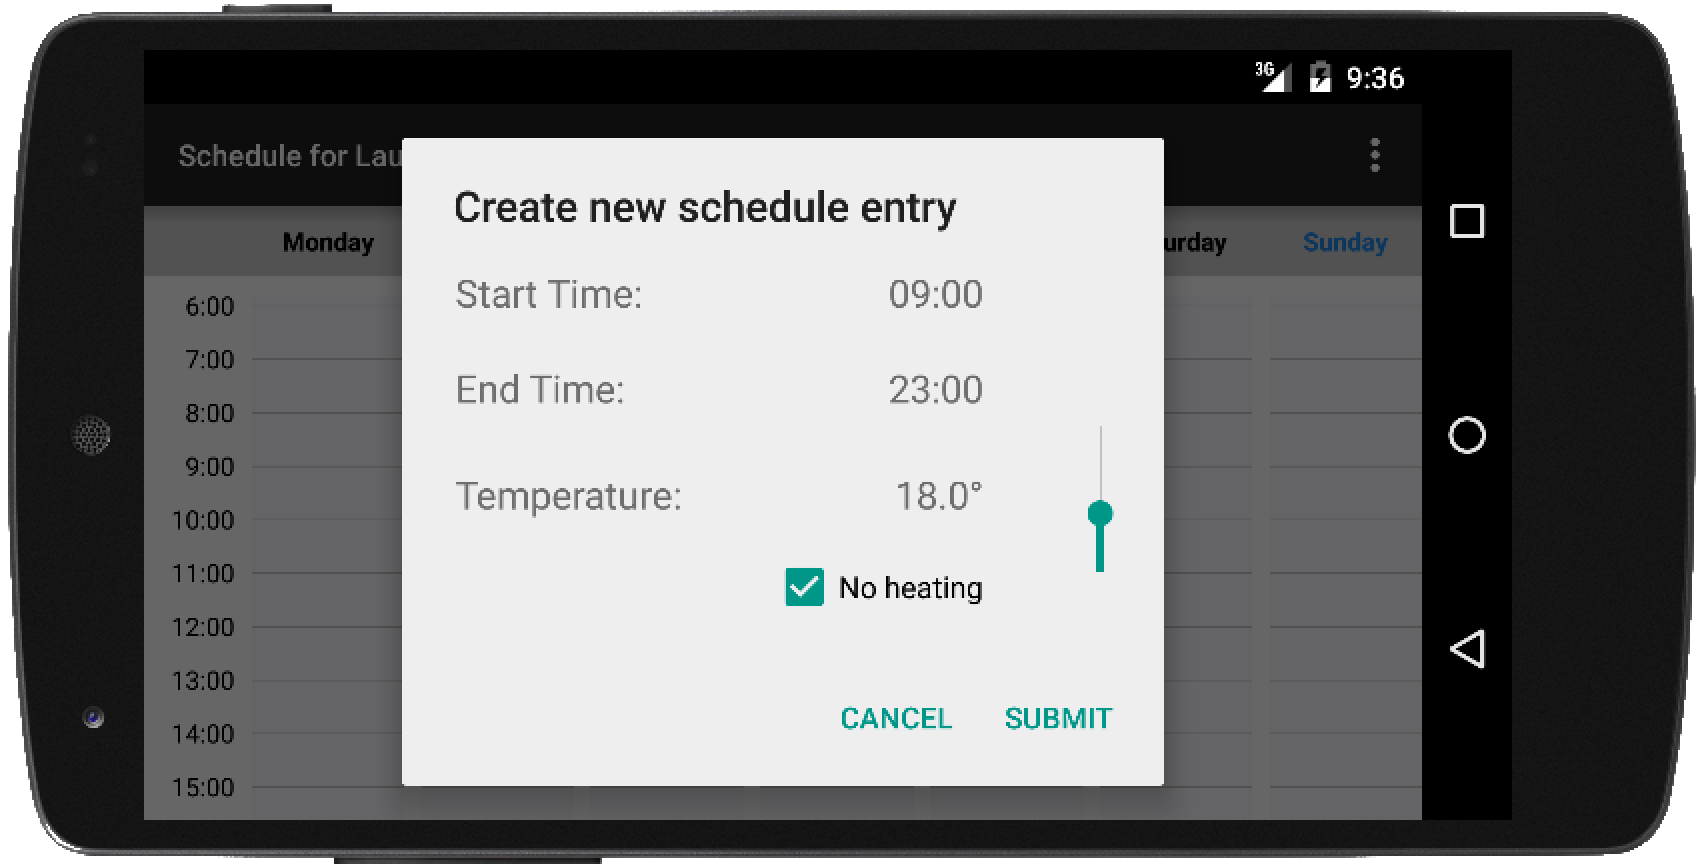
\includegraphics[width=0.8\textwidth]{images/new_schedule_entry.png}
	\end{center}
	\caption{The popup for adding a new heating schedule entry.}
	\label{fig:new_schedule_entry}
\end{figure}

\subsection{Internet Connection}

Having a working Internet connection is one of the prerequisites of the application. Without it, the application is unable to propagate any changes performed on the local database to the database on the server, as well as get any updates from the server's database. That is why we implemented a connectivity check that runs in the background of the application. Every few seconds the application checks if there is a working Internet connection.
If there is not, the action bar of the application turns red and shows the text "No internet connection". In this state the local database is essentially frozen. The user is unable to make any changes to it before he regains a working Internet connection. Whenever the user is trying to change something in the system while the action bar is red he will see a popup explaining the situation.
The popup can also be seen when tapping the action bar itself or the small info icon next to it. Figure \ref{fig:no_internet} shows an example of such a popup. In this state the application is unable to update its current temperatures, but the user should be well aware of that fact with the red action bar on top and the text explaining everything. The popup also tells the user when the last update was performed so he knows how old the data being shown to him is. 

\begin{figure}
	\begin{center}
		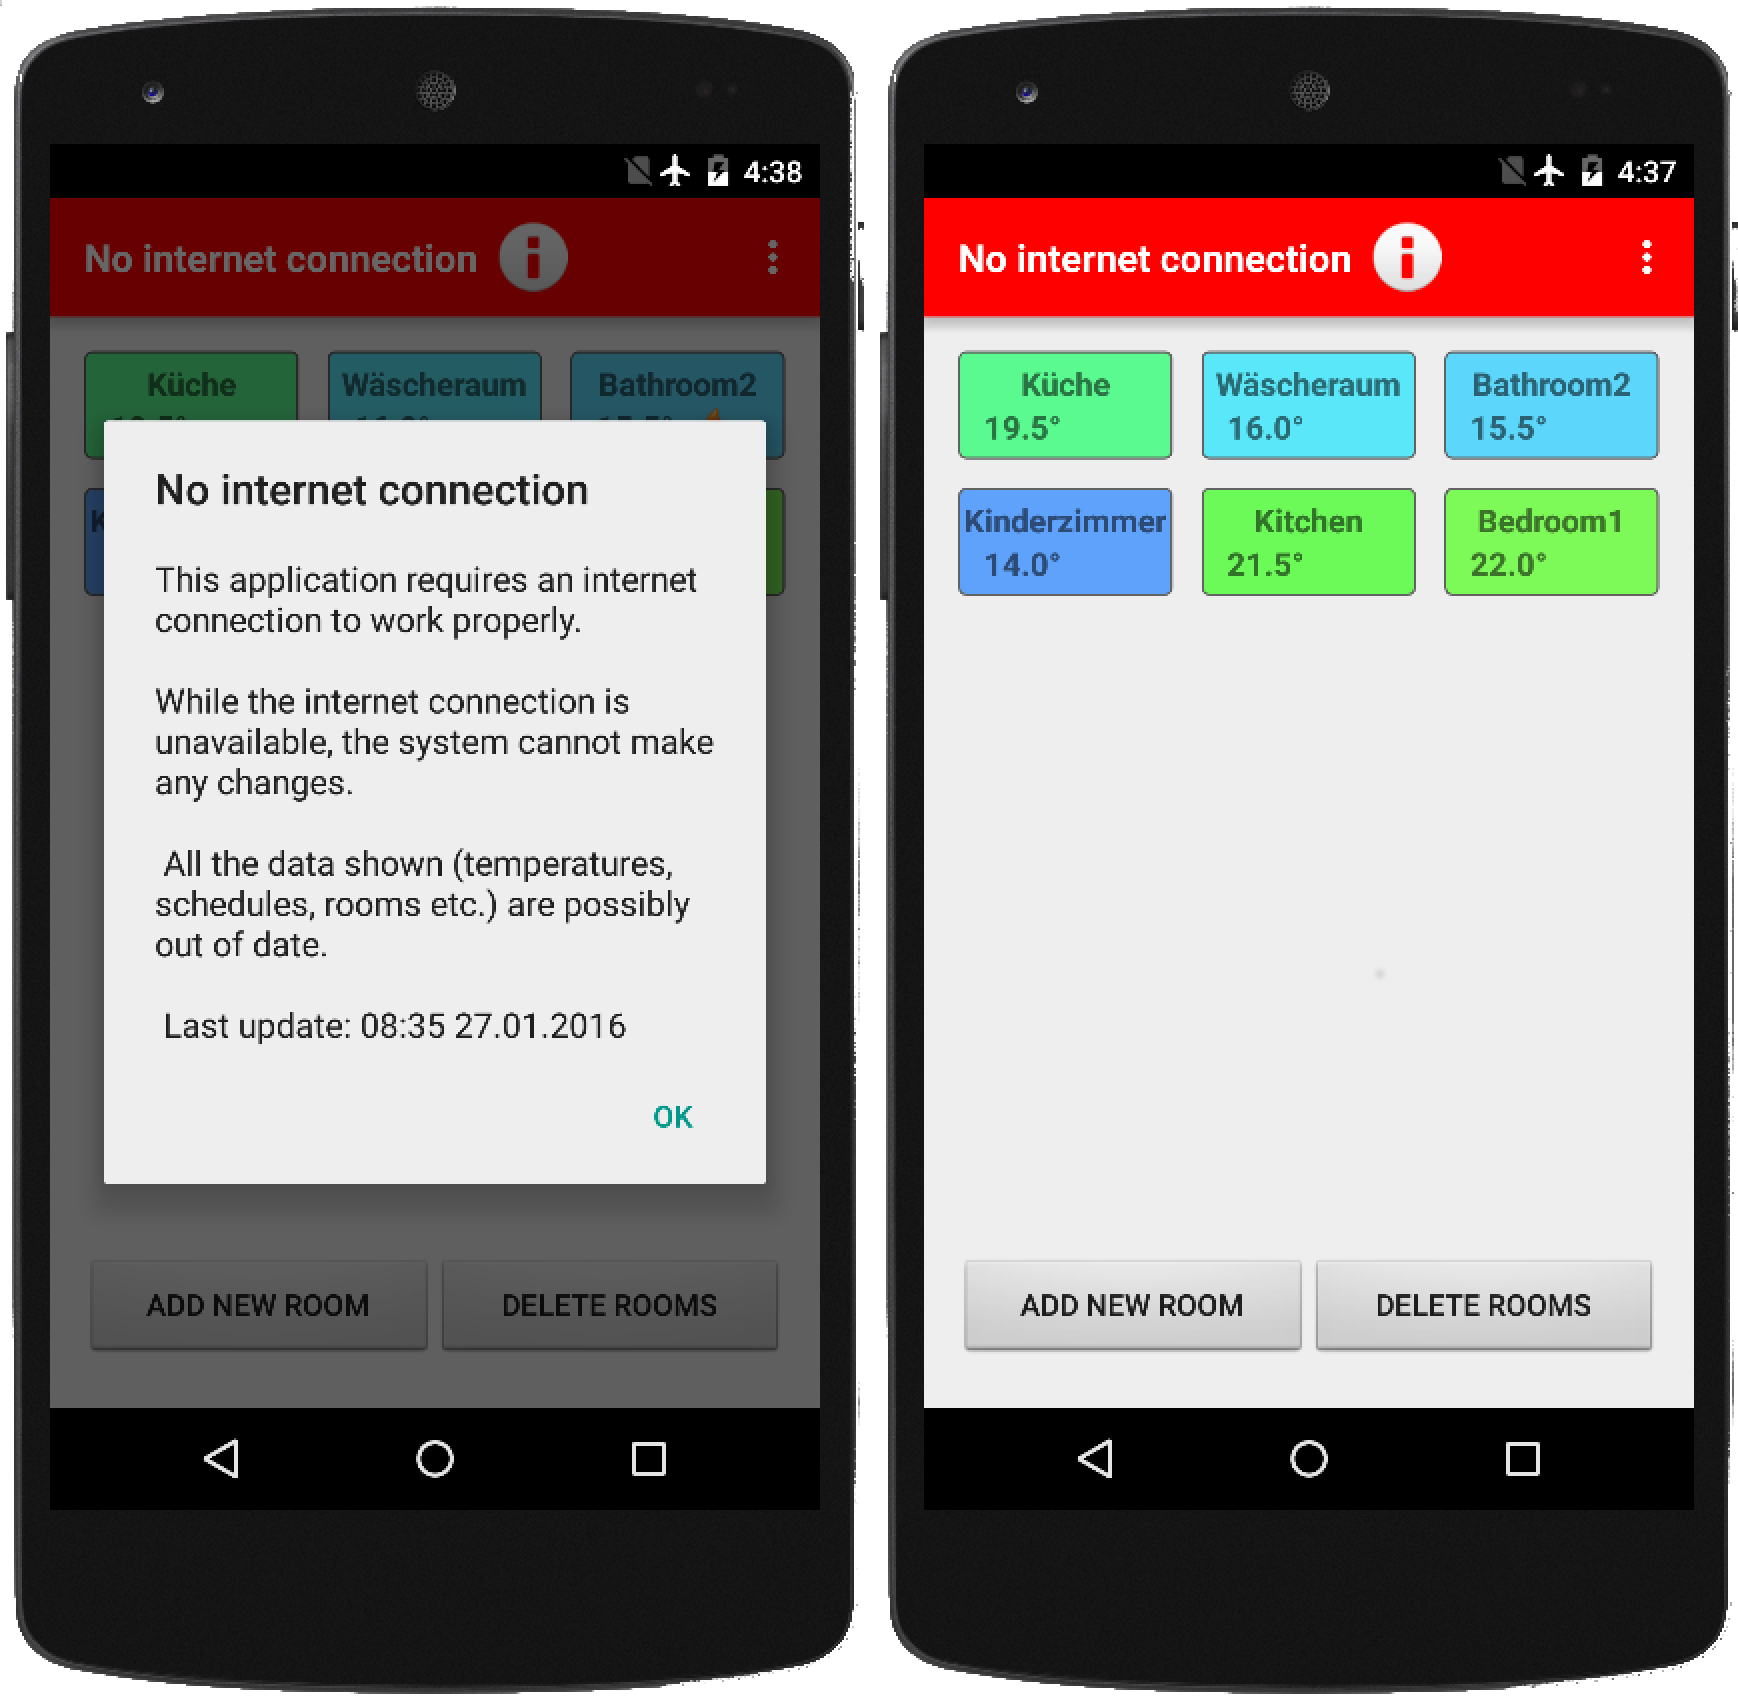
\includegraphics[width=0.8\textwidth]{images/no_internet.png}
	\end{center}
	\caption{The popup when trying to add entities to the system while no Internet connection is available.}
	\label{fig:no_internet}
\end{figure}

\section{Evaluation}

\subsection {Use cases coverage}
Our mobile control application covers most of the use cases introduced in Section \ref{sec:use_cases} adequately. As shown later in some cases we decided to either leave the feature out for simplicity's sake or because it was out of scope for this lab project.

\begin{enumerate}
\item \textbf{Use Case: User wants to install the system}

Covered by the welcome view: The user can easily setup the system using the NFC tags distributed on the raspberry pi and the thermostats with the help of the information displayed on the application.
\item \textbf{Use Case: User feels cold}

Covered by the detail view: The user can adjust the temperature of the room he is currently in using the slider in the detail view.
\item \textbf{Use Case: User wants to save money}

Indirectly covered: The user can choose to set the temperatures lower than usual in order to save money.
\item \textbf{Use Case: User wants to add a room to an existing system}

Covered by the home view: The user can simply add a room using the menu in the upper righthand corner or the button at the bottom of the screen.
\item \textbf{Use Case: User wants to add a thermostat to a room in the system}

Covered by the detail view: The user can add a new thermostat to the currently selected room by simply scanning its NFC tag.
\item \textbf{Use Case: User feels hot}

Covered by the detail view: The user can adjust the temperature of the room he is currently in using the slider in the detail view.
\end{enumerate}

\subsection{User study}
We have conducted a user study with 10 of our fellow students. After giving a brief introduction about the purpose and goal of the application to the participants, we first asked them to try to navigate through the different views of the app. Afterwards they were given a short list of tasks like creating a new room or deleting a thermostat. Each participant was motivated to take note of things that seemed uncomfortable or not intuitive.

For this user study the application was set up in such a way that it is possible to register a dummy residence with a fake RFID. Once registered, the application would automatically add 10 new rooms with randomly chosen but more or less sensible names and add two to four thermostats to each of them. Each thermostat was given an initial dummy value as its current temperature. This was done to be able to collect data for the user study in the case of users which have already set up the system. Some of the tasks also required rooms or thermostats to be already in the system. Of course for the tasks which involved adding new thermostats to the system, actual thermostats were provided with the NFC tags attached to them.

Half of the participants used smart phones not equipped with an NFC adapter for scanning the tags, so they were forced to use the manual entry of RFIDs for the study.

\subsection{Rating}
\label{sec:rating}
After the participants have successfully completed all their tasks, they were asked a series of questions to be answered on a scale of one through five with the following meaning:
\begin{itemize}
\item{1 - Very Bad}
\item{2 - Bad}
\item{3 - Average}
\item{4 - Good}
\item{5 - Very Good}
\end{itemize}

\subsection{Results}
The questions were all phrased in such a way that the scale of Section \ref{sec:rating} was applicable to the question. So most of the questions started with "How well were you able to" and continued from there as follows:
\begin{itemize}
\item{...navigate through the different views of the application?}

8 participants answered with "Very Good", the other two replied with "Good".
\item{...tell the difference between the different views?}

This question focused on designing the views visually in such a way that the user will not get lost while trying to find the feature he is looking for.

All 10 participants answered with "Very Good". 
\item{...quickly see the temperature of any given room and whether it's being heated up or not?}

All 10 participants answered with "Very Good".
\item{...change tomorrow's schedule for a given room?}

6 participants answered with "Very Good", three with "Good" and one "Average".

The biggest problem was figuring out that the schedule of a room could only be changed by going to the settings menu in the room's detail view. Having reached the schedule view for the room most participants were able to complete the task very easily.

\item{...delete a thermostat from a given room?}

All 10 participants answered with "Very Good".
\item{...delete a room from the system?}

All 10 participants answered with "Very Good".
\item{...add a thermostat to a given room?}

5 participants answered with "Very Good", two with "Good" and three with "Average".

All of the participants using a smart phone with a NFC adapter replied with "Very Good" since scanning the tag is very convenient for the user. The manual method still works, but it is rather cumbersome to be able to read the RFID written on the tags.
\item{...add a room to the system?}

All 10 participants answered with "Very Good".

\item{How would you rate the overall impression of the application visually?}

Two participants answered with "Very Good", 4 with "Good" and 4 with "Average".

\item{How would you rate the overall usability of the application?}

8 participants answered with "Very Good", two replied with "Good".

\item{Would you consider using such a heating system in your own home?}

Here the answers were not given in the usual scale but rather as statements. 

Most of the participants considered it not worth the price of exchanging all their thermostats at home and buying a raspberry pi just to maybe save a little bit of money in heating cost. These statements are of course from students which is probably not the best group for such a question, but conducting a bigger user study or even reaching out to users of existing smart heating systems for a questionnaire lies beyond the scope of this project.
\end{itemize}

